% SPDX-License-Identifier: CC-BY-4.0
% Copyright (c) 2026 Jonathan Yantis. Research draft; not submitted.
\documentclass[10pt,letterpaper]{article}
\usepackage[margin=0.70in]{geometry}
\usepackage[T1]{fontenc}
\usepackage{mathptmx,amsmath,amssymb,booktabs,array,ragged2e,xcolor,microtype,xurl,hyperref,fancyhdr,tikz,pgfplots}
\usetikzlibrary{arrows.meta,positioning}
\pgfplotsset{compat=1.18}
\definecolor{studyblue}{RGB}{32,75,103}
\definecolor{studyorange}{RGB}{178,87,28}
\hypersetup{colorlinks=true,urlcolor=studyblue,citecolor=studyblue,linkcolor=black,pdfauthor={Jonathan Yantis},pdftitle={Precision Bluetooth Timing on ESP32-S3: Causal Clock Discipline and Hardware Event Capture}}
\setlength{\parindent}{1em}\setlength{\parskip}{2pt}\setlength{\headheight}{14pt}\setlength{\emergencystretch}{2em}
\widowpenalty=10000\clubpenalty=10000
\pagestyle{fancy}\fancyhf{}\fancyhead[L]{\small Precision Bluetooth Timing on ESP32-S3}\fancyhead[R]{\small Research draft, 22 October 2026}\fancyfoot[C]{\small\thepage}
\newcommand{\ns}{\,\mathrm{ns}}\newcommand{\us}{\,\mu\mathrm{s}}\newcommand{\ms}{\,\mathrm{ms}}
\newcommand{\code}[1]{\texttt{#1}}
\newcolumntype{L}[1]{>{\RaggedRight\arraybackslash}p{#1}}
\renewcommand{\arraystretch}{1.15}
\newcommand{\TrainingEcdf}{(0,0) (0,0.020833333) (1,0.041666667) (1,0.062500000) (2,0.083333333) (4,0.104166667) (7,0.125000000) (8,0.145833333) (9,0.166666667) (18,0.187500000) (21,0.208333333) (30,0.229166667) (31,0.250000000) (31,0.270833333) (32,0.291666667) (32,0.312500000) (33,0.333333333) (43,0.354166667) (56,0.375000000) (57,0.395833333) (57,0.416666667) (58,0.437500000) (59,0.458333333) (61,0.479166667) (62,0.500000000) (62,0.520833333) (65,0.541666667) (67,0.562500000) (68,0.583333333) (70,0.604166667) (81,0.625000000) (87,0.645833333) (88,0.666666667) (94,0.687500000) (95,0.708333333) (98,0.729166667) (100,0.750000000) (107,0.770833333) (109,0.791666667) (112,0.812500000) (114,0.833333333) (115,0.854166667) (118,0.875000000) (127,0.895833333) (142,0.916666667) (163,0.937500000) (168,0.958333333) (173,0.979166667) (194,1.000000000)}
\newcommand{\TraceLimit}{500}
\newcommand{\GapShade}{\addplot[draw=none,fill=gray!18,forget plot] coordinates {(615.679109938,-500) (660,-500) (660,500) (615.679109938,500)}\closedcycle;\node[rotate=90,font=\scriptsize,text=gray!70!black] at (axis cs:637.839554969,0) {no PPS records};}
\newcommand{\AbstractResults}{In a prespecified 660 s window, 616 PPS records were retained: 615 eligible observations had mean $42.346\ns$, uncentered RMS $110.801\ns$ and maximum absolute residual 402 ns. One row was ineligible and a disabled collection ending left 44 nominal one-second opportunities unrecorded. The original run failed its required post-window fence; conditional precision does not establish continuous availability.}
\newcommand{\ProtocolResults}{The new window is exactly $660\times16{,}000{,}000$ nominal receiver-counter ticks, with an inclusive start and exclusive end in one capture epoch. Every recorded in-window validity class is retained. Acquisition took 54.081 s; a 10 s proof interval retained nine full CRC-protected transmit pairs, with one incomplete/CRC-rejected envelope and two dropped/two expired diagnostic records. The collector continued to 689.983 s after the native start but failed the original 690 s collection/drain deadline without its required post-window PPS sequence fence. Its original status remains FAILED. No restart, backfill or retuning is part of this cohort.}
\newcommand{\LongResults}{The fixed 660 s experiment retained 616 records with zero interior software sequence gaps or duplicates. Of these, 615 meet the full reference/diagnostic eligibility rule; one does not. Eligible mean is $42.346\ns$, RMS $110.801\ns$, standard deviation $102.390\ns$, absolute P50/P95/P99 $78/217/278\ns$ and maximum $402\ns$ (signed range $-311$ to $402\ns$). The eligible first-to-last span is 614.000253 s; all recorded edges span 615.000254 s, satisfying the longer-than-ten-minute observation goal while retaining the incomplete ending. The last record occurs 615.679110 s into the window and has diagnostic enabled=false and reference seen/fix/PPS=false, despite map-valid=true and reason=0. Its numeric phase, 125 ns, is not an eligible residual. No later PPS record was available for the remaining 44.320890 s; 208 of 1992 shadow responses report disabled collection. The required post-window sequence fence is absent and native-population completeness is unestablished. This is a diagnostic collection/availability failure; physical GNSS or PPS failure is not established. UI/session ownership can disable the collector, but the exact trigger is unknown. At nominal 1 Hz, opportunity accounting is $660=615$ eligible $+1$ invalid $+44$ unrecorded, giving 93.182\% nominal eligible coverage. This is a declared opportunity model, not independently enumerated physical pulses. The original FAILED status and all empty polls, losses and disabled responses remain in the supplement.}
\newcommand{\LongTrace}{(0.678856250,97) (1.678856625,126) (2.678857000,34) (3.678857375,50) (4.678857750,6) (5.678858125,-11) (6.678858563,98) (7.678858938,220) (8.678859313,179) (9.678859687,41) (10.678860063,-52) (11.678860500,-27) (12.678860875,14) (13.678861313,106) (14.678861625,56) (15.678862000,109) (16.678862438,173) (17.678862813,230) (18.678863187,80) (19.678863562,42) (20.678863938,-17) (21.678864375,114) (22.678864750,104) (23.678865125,200) (24.678865500,193) (25.678865937,154) (26.678866312,136) (27.678866750,54) (28.678867125,201) (29.678867437,98) (30.678867875,147) (31.678868250,94) (32.678868625,71) (33.678869000,64) (34.678869375,-22) (35.678869750,-59) (36.678870125,-59) (37.678870563,187) (38.678870938,183) (39.678871313,147) (40.678871750,278) (41.678872125,149) (42.678872500,-173) (43.678872875,-125) (44.678873313,-162) (45.678873688,127) (46.678874063,268) (47.678874437,173) (48.678874875,246) (49.678875250,249) (50.678875625,-74) (51.678876063,-43) (52.678876438,-39) (53.678876813,-79) (54.678877187,48) (55.678877562,-11) (56.678878000,135) (57.678878375,94) (58.678878750,-25) (59.678879188,31) (60.678879563,154) (61.678879937,88) (62.678880312,125) (63.678880750,167) (64.678881125,115) (65.678881500,-10) (66.678881875,-94) (67.678882250,-311) (68.678882625,-97) (69.678883000,38) (70.678883375,101) (71.678883750,27) (72.678884188,-71) (73.678884625,14) (74.678885000,-53) (75.678885375,-121) (76.678885750,-42) (77.678886125,-80) (78.678886562,99) (79.678886937,108) (80.678887312,211) (81.678887687,123) (82.678888125,28) (83.678888500,97) (84.678888875,31) (85.678889250,-53) (86.678889625,-47) (87.678890063,110) (88.678890438,206) (89.678890813,277) (90.678891187,92) (91.678891562,11) (92.678892000,40) (93.678892375,50) (94.678892750,-113) (95.678893187,113) (96.678893562,156) (97.678893938,54) (98.678894313,62) (99.678894750,68) (100.678895125,-70) (101.678895500,-104) (102.678895875,-105) (103.678896250,-115) (104.678896625,-104) (105.678897000,102) (106.678897437,56) (107.678897812,26) (108.678898250,39) (109.678898625,5) (110.678899000,-44) (111.678899375,89) (112.678899750,-1) (113.678900188,124) (114.678900563,51) (115.678900938,60) (116.678901375,167) (117.678901750,-8) (118.678902125,-213) (119.678902500,-64) (120.678902875,-82) (121.678903312,-4) (122.678903687,128) (123.678904062,129) (124.678904437,138) (125.678904812,36) (126.678905188,66) (127.678905625,-37) (128.678906000,-94) (129.678906375,-55) (130.678906750,-105) (131.678907125,6) (132.678907500,-33) (133.678907937,93) (134.678908312,-21) (135.678908688,8) (136.678909125,78) (137.678909500,19) (138.678909875,4) (139.678910250,14) (140.678910625,-97) (141.678911062,88) (142.678911438,-78) (143.678911812,105) (144.678912250,215) (145.678912625,42) (146.678913000,-11) (147.678913438,107) (148.678913813,93) (149.678914125,-95) (150.678914500,-217) (151.678914937,0) (152.678915313,11) (153.678915687,-79) (154.678916063,-72) (155.678916437,26) (156.678916875,106) (157.678917313,-129) (158.678917687,-141) (159.678918063,4) (160.678918437,-167) (161.678918813,-125) (162.678919187,45) (163.678919625,122) (164.678920000,70) (165.678920375,121) (166.678920812,127) (167.678921188,151) (168.678921562,206) (169.678921938,145) (170.678922312,97) (171.678922688,162) (172.678923125,120) (173.678923500,91) (174.678923875,46) (175.678924250,8) (176.678924688,46) (177.678925063,36) (178.678925437,12) (179.678925813,34) (180.678926187,-11) (181.678926625,-124) (182.678926937,-47) (183.678927375,-4) (184.678927750,-151) (185.678928125,-53) (186.678928563,93) (187.678928937,15) (188.678929313,-9) (189.678929687,-138) (190.678930063,54) (191.678930500,-22) (192.678930875,44) (193.678931250,72) (194.678931625,59) (195.678932000,139) (196.678932375,81) (197.678932812,14) (198.678933188,98) (199.678933562,132) (200.678934000,110) (201.678934375,31) (202.678934750,-39) (203.678935125,-42) (204.678935500,-97) (205.678935875,-127) (206.678936250,-77) (207.678936625,-136) (208.678937063,-157) (209.678937437,-102) (210.678937813,-122) (211.678938187,-50) (212.678938625,83) (213.678939000,98) (214.678939375,29) (215.678939750,35) (216.678940187,116) (217.678940563,-8) (218.678940937,-111) (219.678941375,0) (220.678941750,-69) (221.678942125,70) (222.678942500,154) (223.678942938,38) (224.678943312,59) (225.678943688,20) (226.678944062,-11) (227.678944438,40) (228.678944875,-29) (229.678945250,-173) (230.678945625,-133) (231.678946000,-56) (232.678946438,-212) (233.678946812,-55) (234.678947250,-14) (235.678947625,57) (236.678948000,196) (237.678948375,-11) (238.678948750,85) (239.678949187,104) (240.678949563,80) (241.678949937,26) (242.678950313,-162) (243.678950750,-176) (244.678951125,-182) (245.678951500,-166) (246.678951875,-48) (247.678952313,23) (248.678952687,121) (249.678953062,98) (250.678953438,42) (251.678953812,-91) (252.678954188,-60) (253.678954625,64) (254.678955000,13) (255.678955375,-114) (256.678955750,-8) (257.678956187,44) (258.678956562,40) (259.678956938,51) (260.678957313,26) (261.678957687,-12) (262.678958062,-52) (263.678958500,-39) (264.678958875,-33) (265.678959313,-96) (266.678959625,121) (267.678960062,140) (268.678960437,50) (269.678960875,127) (270.678961250,123) (271.678961625,122) (272.678962000,74) (273.678962375,81) (274.678962750,47) (275.678963125,107) (276.678963562,144) (277.678963937,-49) (278.678964312,8) (279.678964688,-11) (280.678965125,-156) (281.678965500,-81) (282.678965875,-15) (283.678966312,126) (284.678966688,127) (285.678967063,133) (286.678967437,-33) (287.678967875,93) (288.678968188,12) (289.678968625,28) (290.678969000,42) (291.678969375,189) (292.678969750,47) (293.678970187,120) (294.678970563,-66) (295.678970938,-52) (296.678971312,34) (297.678971687,-73) (298.678972125,125) (299.678972500,234) (300.678972875,179) (301.678973312,17) (302.678973687,-102) (303.678974125,-50) (304.678974500,4) (305.678974875,-35) (306.678975250,-27) (307.678975687,90) (308.678976062,92) (309.678976438,43) (310.678976875,134) (311.678977250,66) (312.678977687,181) (313.678978125,219) (314.678978500,57) (315.678978875,-76) (316.678979313,73) (317.678979750,24) (318.678980125,169) (319.678980500,180) (320.678980938,107) (321.678981313,92) (322.678981688,-5) (323.678982062,9) (324.678982562,151) (325.678983000,42) (326.678983375,125) (327.678983750,143) (328.678984188,132) (329.678984625,16) (330.678985062,-6) (331.678985437,-131) (332.678985875,79) (333.678986250,47) (334.678986688,93) (335.678987063,71) (336.678987437,14) (337.678987875,100) (338.678988312,177) (339.678988750,78) (340.678989125,-107) (341.678989563,-33) (342.678989937,173) (343.678990375,116) (344.678990812,76) (345.678991250,-36) (346.678991688,-51) (347.678992063,84) (348.678992500,108) (349.678992875,31) (350.678993312,-24) (351.678993687,11) (352.678994125,-159) (353.678994563,-62) (354.678995000,68) (355.678995375,66) (356.678995812,-81) (357.678996250,119) (358.678996625,27) (359.678997063,147) (360.678997500,-61) (361.678997938,65) (362.678998375,251) (363.678998750,117) (364.678999187,200) (365.678999625,51) (366.679000062,77) (367.679000438,85) (368.679000875,100) (369.679001313,157) (370.679001750,217) (371.679002125,-45) (372.679002562,149) (373.679003000,90) (374.679003438,16) (375.679003813,90) (376.679004250,67) (377.679004688,-84) (378.679005125,123) (379.679005500,40) (380.679006000,79) (381.679006437,88) (382.679006875,218) (383.679007250,115) (384.679007688,98) (385.679008062,148) (386.679008562,322) (387.679008937,95) (388.679009375,97) (389.679009812,42) (390.679010250,45) (391.679010688,3) (392.679011125,35) (393.679011563,118) (394.679012000,266) (395.679012375,95) (396.679012812,44) (397.679013250,25) (398.679013688,49) (399.679014125,19) (400.679014563,-87) (401.679015000,18) (402.679015438,8) (403.679015875,78) (404.679016312,222) (405.679016750,95) (406.679017187,-44) (407.679017625,58) (408.679018000,17) (409.679018438,44) (410.679018875,-66) (411.679019312,-9) (412.679019750,153) (413.679020187,10) (414.679020625,-21) (415.679021062,227) (416.679021500,316) (417.679021938,104) (418.679022375,-47) (419.679022813,27) (420.679023250,19) (421.679023687,17) (422.679024125,-40) (423.679024562,46) (424.679025000,173) (425.679025438,144) (426.679025875,142) (427.679026313,104) (428.679026688,154) (429.679027125,10) (430.679027562,5) (431.679028000,-153) (432.679028500,-28) (433.679028875,-102) (434.679029313,-155) (435.679029750,-170) (436.679030188,34) (437.679030625,73) (438.679031125,240) (439.679031500,91) (440.679031937,186) (441.679032375,176) (442.679032812,118) (443.679033312,335) (444.679033688,176) (445.679034125,-14) (446.679034563,224) (447.679035000,42) (448.679035437,47) (449.679035875,-28) (450.679036312,38) (451.679036750,-25) (452.679037188,36) (453.679037625,-134) (454.679038063,16) (455.679038500,39) (456.679038938,63) (457.679039375,-62) (458.679039812,38) (459.679040250,-1) (460.679040687,198) (461.679041187,256) (462.679041625,174) (463.679042000,-67) (464.679042438,112) (465.679042875,67) (466.679043375,47) (467.679043813,-60) (468.679044187,89) (469.679044625,-64) (470.679045062,77) (471.679045562,159) (472.679046000,57) (473.679046375,34) (474.679046813,66) (475.679047313,28) (476.679047750,34) (477.679048187,-59) (478.679048625,-32) (479.679049062,24) (480.679049437,-146) (481.679049937,90) (482.679050375,153) (483.679050813,187) (484.679051250,18) (485.679051688,96) (486.679052125,-19) (487.679052562,127) (488.679053000,-164) (489.679053437,-183) (490.679053875,-76) (491.679054312,14) (492.679054750,-8) (493.679055188,31) (494.679055625,138) (495.679056063,164) (496.679056563,-37) (497.679057000,96) (498.679057437,99) (499.679057875,0) (500.679058312,94) (501.679058750,-123) (502.679059188,-16) (503.679059625,45) (504.679060063,57) (505.679060500,-37) (506.679060938,107) (507.679061375,98) (508.679061875,55) (509.679062312,51) (510.679062750,46) (511.679063187,-58) (512.679063625,96) (513.679064062,221) (514.679064500,149) (515.679065000,143) (516.679065437,70) (517.679065875,88) (518.679066313,105) (519.679066688,-238) (520.679067187,43) (521.679067625,35) (522.679068063,-30) (523.679068562,-6) (524.679068938,13) (525.679069375,-27) (526.679069812,38) (527.679070313,120) (528.679070750,123) (529.679071187,108) (530.679071625,153) (531.679072125,144) (532.679072562,-77) (533.679073000,26) (534.679073438,3) (535.679073875,65) (536.679074375,244) (537.679074812,81) (538.679075250,185) (539.679075688,-17) (540.679076125,-63) (541.679076562,-110) (542.679077000,-3) (543.679077438,-102) (544.679077937,160) (545.679078375,194) (546.679078813,294) (547.679079250,237) (548.679079688,101) (549.679080187,-23) (550.679080625,-73) (551.679081063,-72) (552.679081500,-6) (553.679081937,23) (554.679082375,130) (555.679082813,55) (556.679083250,47) (557.679083750,111) (558.679084188,77) (559.679084687,42) (560.679085063,-40) (561.679085562,-24) (562.679086000,103) (563.679086438,-23) (564.679086875,-13) (565.679087312,157) (566.679087750,161) (567.679088188,47) (568.679088625,162) (569.679089062,133) (570.679089563,-14) (571.679090000,-72) (572.679090438,-45) (573.679090937,93) (574.679091375,181) (575.679091813,123) (576.679092250,40) (577.679092687,273) (578.679093125,-56) (579.679093625,-40) (580.679094062,-39) (581.679094500,-23) (582.679094938,11) (583.679095437,167) (584.679095875,-7) (585.679096312,10) (586.679096750,-114) (587.679097188,119) (588.679097687,184) (589.679098125,197) (590.679098563,-1) (591.679099062,217) (592.679099500,220) (593.679099938,52) (594.679100375,129) (595.679100875,176) (596.679101313,128) (597.679101750,-24) (598.679102188,-11) (599.679102625,-64) (600.679103125,-31) (601.679103563,-57) (602.679104000,-67) (603.679104500,152) (604.679104938,189) (605.679105375,91) (606.679105812,402) (607.679106250,74) (608.679106750,-114) (609.679107187,-117) (610.679107625,-57) (611.679108125,-118) (612.679108563,-137) (613.679109000,-84) (614.679109500,52) (nan,nan)}
\newcommand{\LongEcdf}{(0,0) (0,0.001626016) (0,0.003252033) (0,0.004878049) (1,0.006504065) (1,0.008130081) (1,0.009756098) (3,0.011382114) (3,0.013008130) (3,0.014634146) (4,0.016260163) (4,0.017886179) (4,0.019512195) (4,0.021138211) (4,0.022764228) (5,0.024390244) (5,0.026016260) (5,0.027642276) (6,0.029268293) (6,0.030894309) (6,0.032520325) (6,0.034146341) (6,0.035772358) (7,0.037398374) (8,0.039024390) (8,0.040650407) (8,0.042276423) (8,0.043902439) (8,0.045528455) (8,0.047154472) (8,0.048780488) (8,0.050406504) (9,0.052032520) (9,0.053658537) (9,0.055284553) (10,0.056910569) (10,0.058536585) (10,0.060162602) (10,0.061788618) (11,0.063414634) (11,0.065040650) (11,0.066666667) (11,0.068292683) (11,0.069918699) (11,0.071544715) (11,0.073170732) (11,0.074796748) (11,0.076422764) (11,0.078048780) (11,0.079674797) (11,0.081300813) (12,0.082926829) (12,0.084552846) (12,0.086178862) (13,0.087804878) (13,0.089430894) (13,0.091056911) (14,0.092682927) (14,0.094308943) (14,0.095934959) (14,0.097560976) (14,0.099186992) (14,0.100813008) (14,0.102439024) (14,0.104065041) (14,0.105691057) (15,0.107317073) (15,0.108943089) (16,0.110569106) (16,0.112195122) (16,0.113821138) (16,0.115447154) (17,0.117073171) (17,0.118699187) (17,0.120325203) (17,0.121951220) (17,0.123577236) (18,0.125203252) (18,0.126829268) (19,0.128455285) (19,0.130081301) (19,0.131707317) (19,0.133333333) (20,0.134959350) (21,0.136585366) (21,0.138211382) (22,0.139837398) (22,0.141463415) (23,0.143089431) (23,0.144715447) (23,0.146341463) (23,0.147967480) (23,0.149593496) (24,0.151219512) (24,0.152845528) (24,0.154471545) (24,0.156097561) (24,0.157723577) (25,0.159349593) (25,0.160975610) (25,0.162601626) (26,0.164227642) (26,0.165853659) (26,0.167479675) (26,0.169105691) (26,0.170731707) (27,0.172357724) (27,0.173983740) (27,0.175609756) (27,0.177235772) (27,0.178861789) (27,0.180487805) (28,0.182113821) (28,0.183739837) (28,0.185365854) (28,0.186991870) (28,0.188617886) (29,0.190243902) (29,0.191869919) (30,0.193495935) (31,0.195121951) (31,0.196747967) (31,0.198373984) (31,0.200000000) (31,0.201626016) (31,0.203252033) (32,0.204878049) (33,0.206504065) (33,0.208130081) (33,0.209756098) (33,0.211382114) (34,0.213008130) (34,0.214634146) (34,0.216260163) (34,0.217886179) (34,0.219512195) (34,0.221138211) (35,0.222764228) (35,0.224390244) (35,0.226016260) (35,0.227642276) (36,0.229268293) (36,0.230894309) (36,0.232520325) (36,0.234146341) (37,0.235772358) (37,0.237398374) (37,0.239024390) (38,0.240650407) (38,0.242276423) (38,0.243902439) (38,0.245528455) (38,0.247154472) (39,0.248780488) (39,0.250406504) (39,0.252032520) (39,0.253658537) (39,0.255284553) (39,0.256910569) (40,0.258536585) (40,0.260162602) (40,0.261788618) (40,0.263414634) (40,0.265040650) (40,0.266666667) (40,0.268292683) (40,0.269918699) (41,0.271544715) (42,0.273170732) (42,0.274796748) (42,0.276422764) (42,0.278048780) (42,0.279674797) (42,0.281300813) (42,0.282926829) (42,0.284552846) (42,0.286178862) (42,0.287804878) (43,0.289430894) (43,0.291056911) (43,0.292682927) (44,0.294308943) (44,0.295934959) (44,0.297560976) (44,0.299186992) (44,0.300813008) (44,0.302439024) (45,0.304065041) (45,0.305691057) (45,0.307317073) (45,0.308943089) (45,0.310569106) (46,0.312195122) (46,0.313821138) (46,0.315447154) (46,0.317073171) (47,0.318699187) (47,0.320325203) (47,0.321951220) (47,0.323577236) (47,0.325203252) (47,0.326829268) (47,0.328455285) (47,0.330081301) (47,0.331707317) (47,0.333333333) (48,0.334959350) (48,0.336585366) (49,0.338211382) (49,0.339837398) (50,0.341463415) (50,0.343089431) (50,0.344715447) (50,0.346341463) (50,0.347967480) (51,0.349593496) (51,0.351219512) (51,0.352845528) (51,0.354471545) (51,0.356097561) (52,0.357723577) (52,0.359349593) (52,0.360975610) (52,0.362601626) (52,0.364227642) (53,0.365853659) (53,0.367479675) (53,0.369105691) (54,0.370731707) (54,0.372357724) (54,0.373983740) (55,0.375609756) (55,0.377235772) (55,0.378861789) (55,0.380487805) (56,0.382113821) (56,0.383739837) (56,0.385365854) (56,0.386991870) (57,0.388617886) (57,0.390243902) (57,0.391869919) (57,0.393495935) (57,0.395121951) (57,0.396747967) (58,0.398373984) (58,0.400000000) (59,0.401626016) (59,0.403252033) (59,0.404878049) (59,0.406504065) (59,0.408130081) (60,0.409756098) (60,0.411382114) (60,0.413008130) (61,0.414634146) (62,0.416260163) (62,0.417886179) (62,0.419512195) (63,0.421138211) (63,0.422764228) (64,0.424390244) (64,0.426016260) (64,0.427642276) (64,0.429268293) (64,0.430894309) (65,0.432520325) (65,0.434146341) (66,0.435772358) (66,0.437398374) (66,0.439024390) (66,0.440650407) (66,0.442276423) (66,0.443902439) (67,0.445528455) (67,0.447154472) (67,0.448780488) (67,0.450406504) (68,0.452032520) (68,0.453658537) (69,0.455284553) (70,0.456910569) (70,0.458536585) (70,0.460162602) (70,0.461788618) (71,0.463414634) (71,0.465040650) (71,0.466666667) (72,0.468292683) (72,0.469918699) (72,0.471544715) (72,0.473170732) (73,0.474796748) (73,0.476422764) (73,0.478048780) (73,0.479674797) (74,0.481300813) (74,0.482926829) (74,0.484552846) (76,0.486178862) (76,0.487804878) (76,0.489430894) (77,0.491056911) (77,0.492682927) (77,0.494308943) (77,0.495934959) (77,0.497560976) (78,0.499186992) (78,0.500813008) (78,0.502439024) (78,0.504065041) (79,0.505691057) (79,0.507317073) (79,0.508943089) (79,0.510569106) (80,0.512195122) (80,0.513821138) (80,0.515447154) (81,0.517073171) (81,0.518699187) (81,0.520325203) (81,0.521951220) (81,0.523577236) (82,0.525203252) (83,0.526829268) (84,0.528455285) (84,0.530081301) (84,0.531707317) (85,0.533333333) (85,0.534959350) (87,0.536585366) (88,0.538211382) (88,0.539837398) (88,0.541463415) (88,0.543089431) (89,0.544715447) (89,0.546341463) (90,0.547967480) (90,0.549593496) (90,0.551219512) (90,0.552845528) (91,0.554471545) (91,0.556097561) (91,0.557723577) (91,0.559349593) (92,0.560975610) (92,0.562601626) (92,0.564227642) (93,0.565853659) (93,0.567479675) (93,0.569105691) (93,0.570731707) (93,0.572357724) (93,0.573983740) (94,0.575609756) (94,0.577235772) (94,0.578861789) (94,0.580487805) (94,0.582113821) (95,0.583739837) (95,0.585365854) (95,0.586991870) (95,0.588617886) (96,0.590243902) (96,0.591869919) (96,0.593495935) (96,0.595121951) (97,0.596747967) (97,0.598373984) (97,0.600000000) (97,0.601626016) (97,0.603252033) (97,0.604878049) (97,0.606504065) (98,0.608130081) (98,0.609756098) (98,0.611382114) (98,0.613008130) (98,0.614634146) (98,0.616260163) (98,0.617886179) (99,0.619512195) (99,0.621138211) (100,0.622764228) (100,0.624390244) (101,0.626016260) (101,0.627642276) (102,0.629268293) (102,0.630894309) (102,0.632520325) (102,0.634146341) (102,0.635772358) (103,0.637398374) (104,0.639024390) (104,0.640650407) (104,0.642276423) (104,0.643902439) (104,0.645528455) (104,0.647154472) (105,0.648780488) (105,0.650406504) (105,0.652032520) (105,0.653658537) (106,0.655284553) (106,0.656910569) (107,0.658536585) (107,0.660162602) (107,0.661788618) (107,0.663414634) (107,0.665040650) (108,0.666666667) (108,0.668292683) (108,0.669918699) (109,0.671544715) (110,0.673170732) (110,0.674796748) (110,0.676422764) (111,0.678048780) (111,0.679674797) (112,0.681300813) (113,0.682926829) (113,0.684552846) (114,0.686178862) (114,0.687804878) (114,0.689430894) (114,0.691056911) (115,0.692682927) (115,0.694308943) (115,0.695934959) (116,0.697560976) (116,0.699186992) (117,0.700813008) (117,0.702439024) (118,0.704065041) (118,0.705691057) (118,0.707317073) (119,0.708943089) (119,0.710569106) (120,0.712195122) (120,0.713821138) (120,0.715447154) (121,0.717073171) (121,0.718699187) (121,0.720325203) (121,0.721951220) (122,0.723577236) (122,0.725203252) (122,0.726829268) (123,0.728455285) (123,0.730081301) (123,0.731707317) (123,0.733333333) (123,0.734959350) (123,0.736585366) (124,0.738211382) (124,0.739837398) (125,0.741463415) (125,0.743089431) (125,0.744715447) (125,0.746341463) (125,0.747967480) (126,0.749593496) (126,0.751219512) (127,0.752845528) (127,0.754471545) (127,0.756097561) (127,0.757723577) (127,0.759349593) (127,0.760975610) (128,0.762601626) (128,0.764227642) (129,0.765853659) (129,0.767479675) (129,0.769105691) (130,0.770731707) (131,0.772357724) (132,0.773983740) (132,0.775609756) (133,0.777235772) (133,0.778861789) (133,0.780487805) (134,0.782113821) (134,0.783739837) (135,0.785365854) (136,0.786991870) (136,0.788617886) (137,0.790243902) (138,0.791869919) (138,0.793495935) (138,0.795121951) (139,0.796747967) (140,0.798373984) (141,0.800000000) (142,0.801626016) (143,0.803252033) (143,0.804878049) (144,0.806504065) (144,0.808130081) (144,0.809756098) (145,0.811382114) (146,0.813008130) (147,0.814634146) (147,0.816260163) (147,0.817886179) (148,0.819512195) (149,0.821138211) (149,0.822764228) (149,0.824390244) (151,0.826016260) (151,0.827642276) (151,0.829268293) (152,0.830894309) (153,0.832520325) (153,0.834146341) (153,0.835772358) (153,0.837398374) (154,0.839024390) (154,0.840650407) (154,0.842276423) (154,0.843902439) (155,0.845528455) (156,0.847154472) (156,0.848780488) (157,0.850406504) (157,0.852032520) (157,0.853658537) (159,0.855284553) (159,0.856910569) (160,0.858536585) (161,0.860162602) (162,0.861788618) (162,0.863414634) (162,0.865040650) (162,0.866666667) (164,0.868292683) (164,0.869918699) (166,0.871544715) (167,0.873170732) (167,0.874796748) (167,0.876422764) (167,0.878048780) (169,0.879674797) (170,0.881300813) (173,0.882926829) (173,0.884552846) (173,0.886178862) (173,0.887804878) (173,0.889430894) (173,0.891056911) (174,0.892682927) (176,0.894308943) (176,0.895934959) (176,0.897560976) (176,0.899186992) (177,0.900813008) (179,0.902439024) (179,0.904065041) (180,0.905691057) (181,0.907317073) (181,0.908943089) (182,0.910569106) (183,0.912195122) (183,0.913821138) (184,0.915447154) (185,0.917073171) (186,0.918699187) (187,0.920325203) (187,0.921951220) (189,0.923577236) (189,0.925203252) (193,0.926829268) (194,0.928455285) (196,0.930081301) (197,0.931707317) (198,0.933333333) (200,0.934959350) (200,0.936585366) (201,0.938211382) (206,0.939837398) (206,0.941463415) (211,0.943089431) (212,0.944715447) (213,0.946341463) (215,0.947967480) (217,0.949593496) (217,0.951219512) (217,0.952845528) (218,0.954471545) (219,0.956097561) (220,0.957723577) (220,0.959349593) (221,0.960975610) (222,0.962601626) (224,0.964227642) (227,0.965853659) (230,0.967479675) (234,0.969105691) (237,0.970731707) (238,0.972357724) (240,0.973983740) (244,0.975609756) (246,0.977235772) (249,0.978861789) (251,0.980487805) (256,0.982113821) (266,0.983739837) (268,0.985365854) (273,0.986991870) (277,0.988617886) (278,0.990243902) (294,0.991869919) (311,0.993495935) (316,0.995121951) (322,0.996747967) (335,0.998373984) (402,1.000000000)}
\newcommand{\FigureStatus}{The gray ending extends to the prespecified 660 s boundary and marks unavailable PPS records after diagnostic collection became disabled; it does not prove absence of physical pulses. The final ineligible record is excluded from the residual line.}
\newcommand{\FreshTableRow}{Actual 46,993: fresh 48 validation &48&$-2.08$&99.61&99.59&241\\}
\newcommand{\LongTableRow}{Actual 46,993: fixed 660 s, eligible &615&42.35&110.80&102.39&402\\}
\newcommand{\ResultInterpretation}{The fresh first 48 on 46,993 ns have mean $-2.083\ns$, RMS $99.608\ns$ and maximum 241 ns, with no invalid selected rows or interior gaps; one extra post-selection terminal edge remained unread. Publisher boots differ across both short cohorts and the long run. No variance change is attributed causally to the offset. In the long run, 108 conservatively bracketed in-window S3 quality snapshots are all LOCK\_EST with rolling causal RMS 154--186 ns. These are overlapping recent histories, not the 615 PPS errors, an aggregate causal RMS or proof of continuous lock. Ten complete one-minute blocks have PPS RMS 91.4--131.2 ns; the final partial block has 15 eligible observations and RMS 145.0 ns. Adjacent eligible errors have descriptive lag-one correlation 0.449. We do not infer an independent-sample confidence interval or impute timing through the unobserved ending.}
\newcommand{\NordicComparison}{The new S3 path has conditional RMS 110.801 ns over 615 eligible observations and 93.182\% nominal eligible opportunity coverage, with a disabled/incomplete ending. The historical Nordic path has conditional RMS 62.504 ns over 436 eligible observations and 72.425\% nominal eligible coverage, with invalid references, expiry and a different missingness pattern. These values describe separate source-relative populations, rather than a controlled SoC ranking or continuous output bound.}
\newcommand{\Reproduction}{The 776 PPS rows retain five distinct actual cohorts and the invalid row, alongside scoped internal snapshots and capture-chain aggregates \cite{supplement}. Run \code{python3 tools/verify\_s3\_paper.py --require-long-cohort} from the root with standard-library Python; it recomputes statistics, eligibility and denominators and checks selected-file/source/PDF hashes. The separate \code{tools/verify\_v14.py} reproduces the Nordic population. The edition receipt binds source, PDF, compiler, evidence and page review.}
\newcommand{\ConclusionResults}{The prespecified 660 s experiment retained 615 eligible PPS observations with 110.801 ns RMS over a span exceeding ten minutes, but ended with disabled collection and 44 nominal opportunities unrecorded. Conditional precision therefore coexists with an explicit availability failure.}

\begin{document}
\title{\vspace{-1.5em}Precision Bluetooth Timing on ESP32-S3:\\Causal Clock Discipline and Hardware Event Capture}
\author{Jonathan Yantis\\\small Independent researcher}
\date{22 October 2026\\\small Research draft; not submitted or peer reviewed}
\maketitle
\vspace{-1em}
\begin{abstract}
Bluetooth timing precision depends on which physical event a timestamp represents, how it is associated with a packet, and whether its clock model was available before the scored event. We describe an ESP32-S3 implementation of Precision Time over BLE (PToB), combining controller-derived receive timestamps, a continuous 20 MHz clock, authenticated delayed corrections and causal software clock discipline. A separate 80 MHz hardware-capture observer investigates finer radio events without changing the production estimator. The production receive descriptor has 500 ns coordinate steps; the observer's 12.5 ns counter steps do not remove that quantization. A training-only aggregate-path correction is applied to an estimated relay's advertised timestamp and evaluated by a Nordic nRF52840 receiver against a local PPS witness. \AbstractResults{} Historical Nordic results are compared with their original denominators and endpoint definitions. Synthetic capture tests and a lossy native-radio subset establish working digital capture and a 62.5 ns observed signal grid, but do not establish packet-level RF endpoint identity. The contribution is a reproducible account of conditional relative timing, its calibration and its measurement limits, together with falsifiable requirements for a future authoritative fine-timestamp backend. No calibrated UTC or independently measured output-pin accuracy is claimed.
\end{abstract}
\noindent\footnotesize Copyright \copyright\ 2026 Jonathan Yantis. Original paper, figures and derived evidence: \href{https://creativecommons.org/licenses/by/4.0/}{CC BY 4.0}. Analysis code: MIT.\normalsize

\section{Introduction}
A Bluetooth application callback says when software learned about a packet. A hardware timestamp can instead describe a radio or controller event, allowing the application to deliver a completed time reference later. The distinction is useful only if the timestamp belongs to the exact packet and its endpoint is known. A fast counter sampling an ambiguous radio-enable signal can produce finely spaced numbers without improving the receiver's knowledge of packet arrival.

PToB joins a retained publication's local event timestamp to a later authenticated source reference. The pair disciplines a numerical clock: software latency controls when the pair becomes usable, while capture determines its local coordinate. Source identity, boot, epoch and finite permission fence timing-path changes.

The Meshnology N30 is an S3 receiver and estimated relay without GNSS. Its production clock uses the shared S3 timing core; a separate native observer defaults OFF. A Nordic-based T096 supplies native ADDRESS capture and a local PPS witness downstream. This tests a heterogeneous path while leaving individual receive, transmit and propagation delays unresolved.

We ask how causal discipline uses 500 ns receive coordinates, how a training-only aggregate correction performs on fresh downstream observations, and what native capture establishes about a finer S3 timestamp source. Each question has a separate population and criterion. A relay-publication offset cannot itself improve the upstream receive estimator or replace its causal RMS.

Reference-Broadcast Synchronization uses common physical broadcasts to compare receiver clocks, separating important sender uncertainties \cite{rbs}. FTSP combines MAC-layer timestamps with skew estimation \cite{ftsp}. We adopt the general principles of event timestamping and relative frequency estimation; we do not claim a new synchronization primitive or rank against their different platforms. Bluetooth periodic advertising provides the transport and scheduling context \cite{btcore}; PToB's authenticated correction semantics and clock-quality policy are implementation choices, not a Bluetooth standard service.

\section{Timestamp association and causal clock discipline}\label{sec:method}
\subsection{Events, completed references and time domains}
Let $c_i$ be a receiver counter coordinate for an original packet and let $t_i$ be its later authenticated source reference. The useful observation is $(c_i,t_i)$, together with immutable packet identity, source scope and reference availability time $a_i$. It is not the callback pair $(a_i,t_i)$. A late correction may train future estimates, but cannot retroactively improve the estimate that existed at $c_i$.

The production S3 counter is an increasing 20 MHz GPTimer selected from the crystal clock, giving 50 ns representation steps. Espressif documents selectable GPTimer sources and the interpretation of the configured count resolution \cite{gptimer}. The receive descriptor uses a controller half-slot clock and a descending half-microsecond field. The pinned adapter relates that descriptor to a bracketed controller-clock read in GPTimer coordinates, retains its enclosure and subtracts the implementation's reference normalization. Descriptor steps are ten GPTimer ticks, or 500 ns. Thus 50 ns storage is not 50 ns receive information.

Matching occurs against retained complete advertising-data bytes and a stable, consume-once controller record. A later correction is admitted only within the corresponding authenticated tuple and source scope. Publication number alone is insufficient across boots, epochs, trains or different parents. The original capture prediction is retained before the correction is allowed to update the clock. Expiry, queue loss, refusal and unmatched records are separate from a zero timing error.

\begin{figure}[h]
\centering
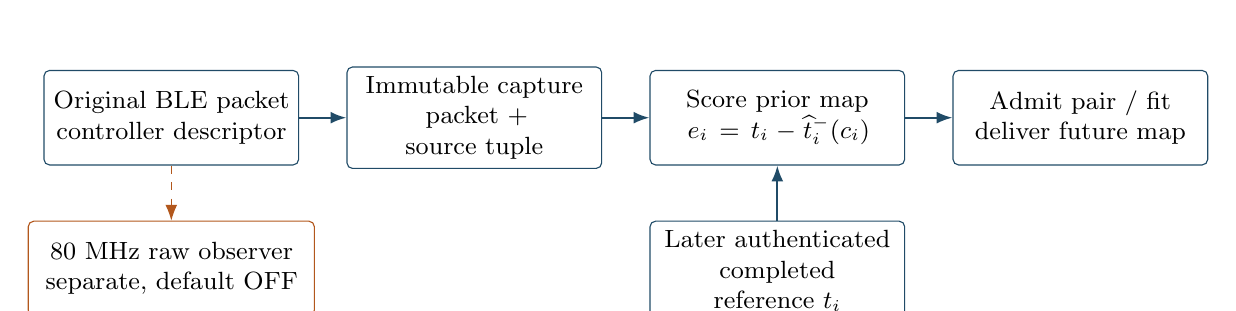
\begin{tikzpicture}[node distance=7mm and 6mm,box/.style={draw=studyblue,rounded corners=2pt,align=center,font=\small,minimum height=12mm,text width=30mm},arr/.style={-{Latex[length=2mm]},draw=studyblue,thick}]
\node[box] (radio) {Original BLE packet\\controller descriptor};
\node[box,right=of radio] (capture) {Immutable capture\\packet + source tuple};
\node[box,right=of capture] (score) {Score prior map\\$e_i=t_i-\widehat t_i^{-}(c_i)$};
\node[box,right=of score] (fit) {Admit pair / fit\\deliver future map};
\draw[arr] (radio)--(capture);\draw[arr] (capture)--(score);\draw[arr] (score)--(fit);
\node[box,below=of score] (later) {Later authenticated\\completed reference $t_i$};
\draw[arr] (later)--(score);
\node[box,below=of radio,draw=studyorange,text width=34mm] (observer) {80 MHz raw observer\\separate, default OFF};
\draw[dashed,draw=studyorange,-{Latex[length=2mm]}] (radio)--(observer);
\end{tikzpicture}
\caption{Causal separation between event capture, delayed knowledge and future clock delivery. The independent observer records candidate evidence without granting timing authority. The figure is an architectural diagram, not an RF delay measurement.}
\label{fig:architecture}
\end{figure}

\subsection{Frequency fitting and bounded phase steering}
The numerical clock projects relative time from a retained base and rate,
\begin{equation}
 \widehat t(c)=\alpha+50(c-c_0)+\rho\frac{c-c_0}{20\times10^6}+s(c),\label{eq:clock}
\end{equation}
where counter units are ticks, $\rho$ is a signed rate correction in ns/s and $s$ is bounded phase steering. Coarse civil-time association is separate from relative phase and frequency. The local crystal is not physically tuned by this software map.

The S3 implementation retains up to 64 physical points. N30 accepts the dense 62.5 ms opportunities rather than thinning them after initial frequency training; a full dense history spans approximately 3.94 s. Rate estimation centers observations within each channel. With $x_i$ measured in seconds and $y_i=t_i-50c_i$ after subtracting an arbitrary origin, the rate fit has the form
\begin{equation}
 \widehat\rho=\frac{\sum_h\sum_{i\in h}(x_i-\bar x_h)(y_i-\bar y_h)}{\sum_h\sum_{i\in h}(x_i-\bar x_h)^2}.\label{eq:rate}
\end{equation}
Repeated-channel evidence prevents a fixed channel offset from being mistaken directly for rate. It does not calibrate channel delay; a changing channel mix can still change phase residuals. Fits require at least two seconds of span, sufficient repeated-channel degrees of freedom and a bounded finite rate. Frequency acceleration is assessed across an observed baseline of at least one second. Warm-up and nonstationary oscillator drift remain possible.

At each completion, the already delivered clock remains continuous. Phase differences up to 1 $\mu$s retain a 1 ppm slew; larger acquisition corrections use a bounded faster slew. Every new reference is scored against its capture-time prior model before training. Recent quality uses 16 physical one-second buckets and includes the causal residual tails, independent of which points enter the fit. At least 16 samples, RMS $\le400\ns$, maximum $<1000\ns$ and a finite sub-microsecond forecast are required for development relative lock; the display then requires settlement. These engineering gates are not a calibrated uncertainty guarantee.

\section{Aggregate correction and prospective experiment}\label{sec:experiment}
\subsection{A deliberately composite calibration}
The optional S3 relay advertises an estimated transmit coordinate derived from a programmed scheduling point. It does not yet expose a calibrated actual RF transmit timestamp. At 1 Mbit/s, a nominal 800 ticks of the 20 MHz counter represents 40 $\mu$s to the selected nominal ADDRESS coordinate. That conversion is an implementation reference convention; an aggregate residual can include S3 receive mapping, clock fitting, transmit estimation, propagation and the downstream receiver's normalization.

We therefore estimate one \emph{path-specific composite} constant, $K$, rather than label it a radio delay. It is bound to publisher, measured root/boot/source scope, receive profile and reference convention. The selected frozen map projects the programmed and nominal ADDRESS coordinates, and their difference is included exactly once:
\begin{equation}
 T_{\rm advertised}=T_{\rm programmed}+K,\qquad
 K=K_{\rm base}(\hbox{frozen map})+K_{\rm residual}.\label{eq:offset}
\end{equation}
Integer projection can yield $K_{\rm base}=39{,}999$ or $40{,}000\ns$ at a nonzero rate; the residual correspondingly changes by one nanosecond. The advertised total must remain the selected $K$. Requiring a literal 40,000 ns projection would reject legitimate rounding rather than detect a wrong profile.

In the first calibration, the first 32 valid observations on nominal $K=40{,}000\ns$ had mean $-6964.781\ns$. Rounding this training mean selected an additional $6965\ns$, hence $K=46{,}965\ns$. The next 32 observations were reserved. Adding 6965 ns to them yields a \emph{counterfactual} RMS of $86.371\ns$ and mean $15.469\ns$; it is not evidence that corrected firmware ran during those samples.

The original nominal calibration had poor diagnostic coverage: 183 dropped and 175 expired records, and only one complete selected arithmetic pair without individual log CRC. Two subsequent verification attempts failed before producing PPS validation data: incomplete selected transmit proof, then a host check that rejected legitimate 39,999 ns rounding. These failures remain separate in the supplement.

The successful actual 46,965 ns observation produced 48/48 valid samples with mean $-27.958\ns$, RMS $85.260\ns$ and maximum absolute residual 194 ns. Ten complete transmit-estimate/path pairs had individual CRC protection and showed exactly 46,965 ns from raw programmed projection to advertised reference, with zero measured capture transport-loss deltas. These 48 observations subsequently selected a further $+28\ns$, giving $K=46{,}993\ns$. Once reused for tuning, they are training history for this final profile, not an independent success population. The next fresh 48 and the longer fixed cohort are evaluated without further retuning.

\subsection{Physical witness and measurement definition}
The downstream Nordic T096 receives the S3 relay and evaluates its delivered map at a locally captured physical PPS. That witness is independent of training the BLE map, but it is not a second calibrated time laboratory. Local PPS-to-UTC association is unavailable in this cohort: the association field is zero and absolute-error output is unavailable. The reported error is a signed fractional-second, source-relative phase,
\begin{equation}
 e_j=\operatorname{wrap}_{[-0.5,0.5)\,s}\{\widehat t_{\rm downstream}(p_j)-\phi_{\rm PPS}\}.\label{eq:pps}
\end{equation}
The downstream receiver retains its existing $+10{,}543\ns$ normalization. It is not re-estimated from this experiment. No physical S3 PPS output pin is measured. Shared source errors can cancel, while fixed receiver, reference and propagation biases may remain.

\subsection{Frozen protocol and analysis}
The hardware operator verifies the selected image/profile and direct parent path, acquires within a fixed deadline, proves the advertised arithmetic and then begins a fixed measurement interval. Acquired time, proof time and cleanup time are reported separately from measurement. The timing observer is OFF. The frozen 46,993 ns profile and analysis are not changed using validation residuals. \ProtocolResults{}

For valid errors, we report signed mean $\bar e$, uncentered RMS $R=\sqrt{\sum e_j^2/n}$, population standard deviation $\sqrt{R^2-\bar e^2}$, nearest-rank absolute quantiles and absolute maximum. The complete trace retains invalid flags and missing sequence positions. A sequence gap denotes missing exported records, not proof of absent physical pulses; an empty poll is not itself a missing PPS. Repeated cursor replies are deduplicated by exact sequence, with conflicting duplicates treated as failures. End counters separately audit unread terminal edges.

\section{Prospective ESP32-S3 path results}\label{sec:results}
\LongResults{}

\begin{figure}[h]
\centering
\begin{tikzpicture}
\begin{axis}[width=0.98\linewidth,height=50mm,xmin=0,xmax=660,ymin=-\TraceLimit,ymax=\TraceLimit,xlabel={Receiver counter time in fixed window (s)},ylabel={Signed relative phase (ns)},grid=major,grid style={gray!15},tick label style={font=\small},label style={font=\small},legend style={font=\small,at={(0.5,1.03)},anchor=south,draw=none},scaled y ticks=false,unbounded coords=jump]
\GapShade
\addplot[studyblue,thin,mark=none] coordinates {\LongTrace};
\addlegendentry{Frozen 46,993 ns profile; no fitted validation offset}
\end{axis}
\end{tikzpicture}
\caption{Every valid relative PPS residual in the fixed measurement cohort, at its actual relative edge coordinate. No mean removal or detrending is applied. Invalid and unavailable opportunities remain counted separately; the line does not imply observation between PPS edges. \FigureStatus{}}
\label{fig:trace}
\end{figure}

\begin{table}[h]
\centering\small
\caption{Separate populations; RMS includes bias. The fixed 660 s accounting is 615 valid $+1$ invalid $+44$ nominal unrecorded opportunities. The shifted row is counterfactual.}\label{tab:results}
\begin{tabular}{L{54mm}rrrrr}
\toprule
Population & $n$ & Mean ns & RMS ns & Std ns & Max $|e|$ ns\\
\midrule
Nominal 40,000: first 32 training &32&$-6964.78$&6965.46&96.98&7163\\
Nominal 40,000: next 32 reserved &32&$-6949.53$&6950.05&84.97&7158\\
Reserved 32 shifted $+6965$ (model)&32&15.47&86.37&84.97&193\\
Actual 46,965: training for $+28$&48&$-27.96$&85.26&80.55&194\\
\FreshTableRow
\LongTableRow
\bottomrule
\end{tabular}
\end{table}

\begin{figure}[h]
\centering
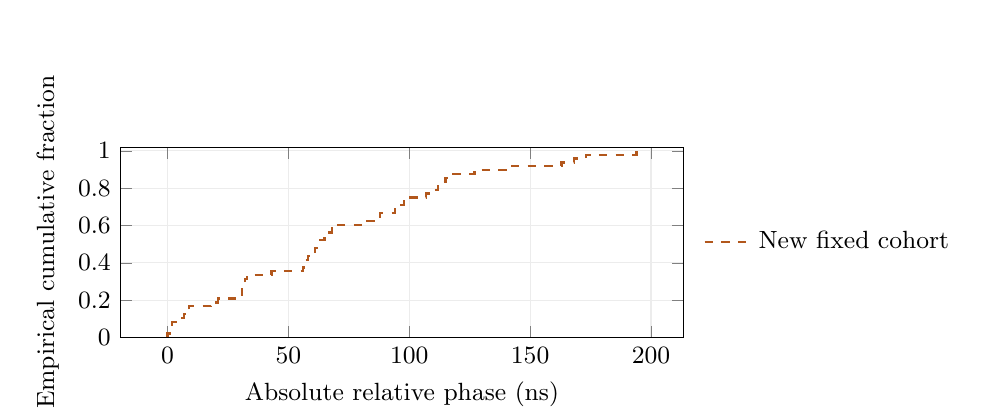
\begin{tikzpicture}
\begin{axis}[width=0.72\linewidth,height=40mm,xlabel={Absolute relative phase (ns)},ylabel={Empirical cumulative fraction},ymin=0,ymax=1.02,grid=major,grid style={gray!15},tick label style={font=\small},label style={font=\small},legend style={font=\small,at={(1.02,0.5)},anchor=west,draw=none}]
\addplot[studyblue,thick,const plot] coordinates {\LongEcdf};\addlegendentry{New fixed cohort}
\addplot[studyorange,dashed,thick,const plot] coordinates {\TrainingEcdf};\addlegendentry{Earlier 48 training}
\end{axis}
\end{tikzpicture}
\caption{Empirical distributions retain each population's raw residual. The earlier 48 selected the additional 28 ns correction and are shown only as calibration context. Neither curve measures the upstream internal Sync RMS or an electrical output. Only 615 eligible observations enter the new-cohort curve; one invalid row and 44 nominal unrecorded opportunities remain in the accounting. This conditional distribution cannot bound errors during disabled collection or identify a causal variance effect of the offset across different boots.}
\end{figure}

\ResultInterpretation{}

\section{Comparison with Nordic timing results}\label{sec:nordic}
\subsection{A hardware endpoint advantage, with its own delay limits}
The nRF52840 exposes a RADIO ADDRESS event for address transmission or reception, a programmable peripheral interconnect (PPI) and TIMER capture tasks. The documented TIMER base frequency is 16 MHz; a capture task copies the running count into a compare/capture register \cite{nordictimer}. PPI can route ADDRESS to TIMER capture without a software callback as the timestamping event, and its signals are synchronized to a 16 MHz clock \cite{nordicppi}. The nominal count step is 62.5 ns. The event name still does not calibrate antenna, detector or propagation delay. Those must be measured or bounded for a physical accuracy claim.

The S3 production path has a different endpoint: controller-derived reception plus a clock-map bracket, followed by estimated relay transmit timing. Its 20 MHz counter is numerically finer than the Nordic counter, but its receive information has 500 ns steps and its transmit estimate is not an actual RF capture. Comparing timer frequencies alone would invert the relevant distinction. The separate 80 MHz observer gives a 12.5 ns latch grid, yet has not established the same packet-level endpoint semantics as ADDRESS.

\begin{table}[h]
\centering\small
\caption{Timestamp mechanisms and demonstrated scope. Nominal tick duration is a representation property, not an accuracy bound.}
\begin{tabular}{L{33mm}L{40mm}L{37mm}L{36mm}}
\toprule
Property & S3 production & S3 observer & Nordic production\\
\midrule
Continuous counter & GPTimer, 20 MHz & MCPWM1, actual 80 MHz & TIMER, 16 MHz\\
Nominal count step &50 ns&12.5 ns&62.5 ns\\
Event information &Descriptor, 500 ns coordinate &RW RX/TX gate candidates &Native RADIO ADDRESS\\
Packet association &Retained bytes + completed tuple &Not yet established &Controller packet capture tuple\\
Transmit reference &Programmed estimate + composite profile &Raw gate only &Native TX capture\\
Current qualification &Conditional relative clock &Digital activity only &Conditional relative clock\\
\bottomrule
\end{tabular}
\end{table}

\subsection{Historical Nordic population, preserved in full}
The available Nordic reference is the separate 12 October V14 one-relay experiment, using application 0.14.43 at source \code{566ea2029c7f} \cite{v14}. It spans 601.576 s and has 602 conservative nominal PPS opportunities. Of 504 observed edges, 436 are reference-valid causal samples; 65 have invalid reference and three have expired maps. Ninety-eight opportunities are unobserved. Thus
\begin{equation}
 602=436\ \hbox{usable}+65\ \hbox{invalid}+3\ \hbox{expired}+98\ \hbox{unobserved}.\label{eq:accounting}
\end{equation}
The 436-sample conditional mean is $-18.417\ns$, RMS $62.504\ns$, standard deviation $59.729\ns$ and maximum absolute residual 191 ns. Valid causal coverage is 72.425\%. The 501-sample all-causal population, including invalid references, has RMS 3.929 ms and maximum absolute residual 19.753 ms. The largest witness gap is 59.017 s. Omitting these denominators would make the conditional 62.5 ns result misleading.

\NordicComparison{}

There is no controlled platform-only performance ranking here. The two experiments have different firmware, dates, path scopes, estimator details and source behavior. Their common unit is nanoseconds, but that does not make their errors exchangeable. The historical Nordic data show what an explicitly associated native endpoint can support under its valid conditions. The new S3 experiment evaluates a complete heterogeneous path after a training-derived aggregate correction. A fair causal comparison of receive backends would use simultaneous common packets, identical reference scopes and an unchanged estimator, with fixed training and heldout intervals.

\subsection{Quantization is a diagnostic, not a complete error model}
For an ideal independent uniformly distributed rounding error with width $q$, RMS is $q/\sqrt{12}$: 144.3 ns for 500 ns, 18.0 ns for 62.5 ns and 3.61 ns for 12.5 ns. These are analytical reference scales. Real packet phase can be correlated with clock scheduling, the clock fit averages multiple samples, and channel effects or path calibration can dominate. A downstream filtered-map PPS RMS below 144.3 ns does not prove that individual S3 packets recovered sub-descriptor phase; it is consistent with smoothing many quantized observations. Conversely, an 80 MHz latch does not guarantee 3.61 ns packet accuracy.

\section{What the 80 MHz hardware observer establishes}\label{sec:observer}
\subsection{Capture-chain controls and observed signal grid}
Espressif specifies an S3 MCPWM capture timer clocked from APB and notes that the capture timer's configurable resolution field is not applicable to this target; the actual resolution is queried \cite{mcpwm}. The technical reference describes a continuously incrementing 32-bit capture counter and per-channel capture registers \cite{s3trm}. The implementation reserves group 1, separate from the LoRa observer's group 0, and fixed GPIO4/5 routes. The driver reports 80 MHz; no independent frequency calibration is implied. Both RX and TX edge records share that counter. At that nominal rate, a 32-bit wrap takes 53.6870912 s, so unambiguous servicing must respect a half-wrap of 26.8435456 s and reject stale/incarnation-mismatched events. A counter restart is a time-domain change, not a new offset sample.

Two slow synthetic GPIO leases issued 16 and eight unique transitions. All expected callbacks, channels and polarities were retained, with no observed invalidity, timeout or console loss. Across the synthetic captures, raw counter values occupied all five residues modulo five; the greatest common divisor of sorted differences was one 80 MHz tick. This establishes that the digital input/capture chain can represent 12.5 ns increments. CPU-issued slow pulses are not an RF phase standard or a test of narrow-pulse completeness.

A distinct 10 s native trial of named RW\_RX\_ON and RW\_TX\_ON signals observed 1262 callbacks: 510 RX and 752 TX. Only 112 unique records were exported, with 1146 interior missing and four terminal unread records. The exported subset has 56 rising and 56 falling edges, a single residue modulo five, and a difference GCD of five raw ticks, or 62.5 ns. This grid differs from the synthetic grid in the same representation and is consistent with a native signal-clock grid. Its finite, lossy subset cannot establish phase jitter or completeness.

\begin{figure}[h]
\centering
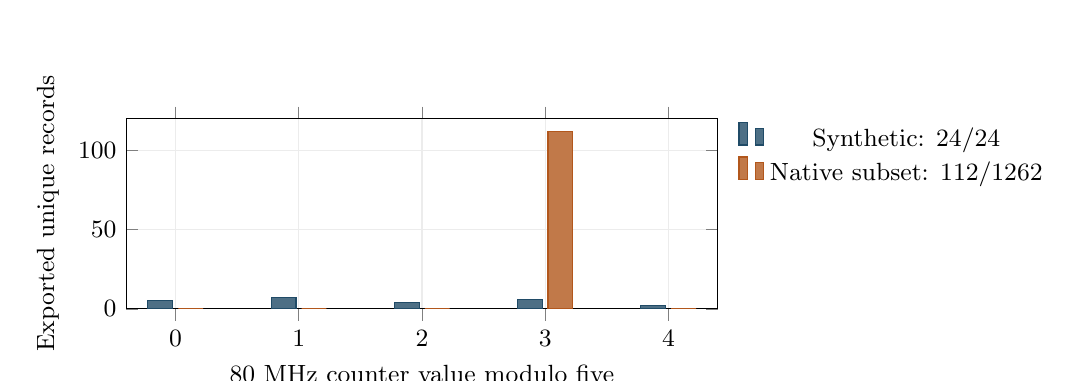
\begin{tikzpicture}
\begin{axis}[ybar,bar width=9pt,width=0.75\linewidth,height=40mm,xlabel={80 MHz counter value modulo five},ylabel={Exported unique records},symbolic x coords={0,1,2,3,4},xtick=data,ymin=0,ymax=120,grid=major,grid style={gray!15},legend style={at={(1.02,0.8)},anchor=west,font=\small,draw=none},tick label style={font=\small},label style={font=\small}]
\addplot[fill=studyblue!80,draw=studyblue] coordinates {(0,5)(1,7)(2,4)(3,6)(4,2)};\addlegendentry{Synthetic: 24/24}
\addplot[fill=studyorange!80,draw=studyorange] coordinates {(0,0)(1,0)(2,0)(3,112)(4,0)};\addlegendentry{Native subset: 112/1262}
\end{axis}
\end{tikzpicture}
\caption{Different observed counter grids. Synthetic counts combine the 16- and eight-edge leases. The native denominator is callback activity; completeness of physical radio events is unknown. A histogram of raw ticks does not identify the packet endpoint.}
\end{figure}

The exported RX gate widths range from approximately 158 $\mu$s to 1.85 ms, and TX widths include approximately 237 $\mu$s and 1.60 ms. These are not a unique packet-address signature. A gate can precede a packet, span a scheduled receive window, end on timeout, or refer to unrelated radio traffic. No selected-packet RF endpoint, path delay or production Sync RMS gain was established. The observed maximum service delay, 16.585 ms, exceeded the 10 ms target, although it remained below half-wrap. Timeout, invalid and error counters were zero in this finite trial; that does not erase its export losses or service-target failure.

\subsection{Why clean software sequences do not prove complete RF capture}
Each MCPWM channel has a capture latch, not a timestamp FIFO. A short pulse can replace a rising-edge value with a falling-edge value before the interrupt handler observes it. Contiguous software callback numbers prove that the observed callbacks were exported; they cannot detect every event lost before the callback. Rising-only trials and independent input counts can probe this failure mode, but cannot independently establish the signal's RF semantics. Similarly, a signal name from the SDK GPIO matrix is a routing lead, not documentation of a calibrated ADDRESS-equivalent event.

\section{A falsifiable path to an authoritative fine backend}\label{sec:next}
A fine backend must identify a physical event, not merely change count units. The next observer-only packet/window journal must retain complete advertising-data bytes and CRC, original descriptor/controller metadata, capture incarnation, event/channel provenance, authentication stage, all candidate edges and every refusal or history gap. Selection must be independent of residual, RSSI and pulse width, with no retrospective nearest-edge rule.

For receive, a fine CURRENT bracket around a legacy GPTimer read locates a search interval; its microsecond enclosure cannot become a nanosecond phase bridge. The window must mature and freeze before ring overwrite. Missing history, delayed callbacks, ambiguity, overflow, unsupported metadata and timeout remain unavailable associations. A callback sequence fence does not establish physical completeness.

For transmit, copy the exact selected frozen advertising bank and programmed-map snapshot independently of bulk logging. The downstream T096 audit must match source/parent boots and epochs, train, publication, event, channel and complete-advertising-data CRC. A correction-completion record is not an independent radio observation; local capture epochs on different devices are separate namespaces.

\begin{table}[h]
\centering\small
\caption{Required evidence before a production fine-timestamp claim. Each row can fail independently; activity alone does not pass later rows.}
\begin{tabular}{L{33mm}L{111mm}}
\toprule
Question & Falsifiable observation / rejection condition\\
\midrule
Does an edge belong to this packet? &Exact immutable packet match plus all candidates in a frozen interval; retain none/multiple, gaps and reused edges.\\
What physical endpoint is it? &Compare rising/falling edges against an independent RF-correlated reference while varying real PDU airtime; include empty, failed and other-traffic windows.\\
Is conversion delay stable? &Measure polarity and endpoint delay by PHY/length/channel with independent timing; disclose temperature, oscillator and propagation assumptions.\\
Does the estimator improve? &Freeze endpoint rule/delay on training only; compare the unchanged causal estimator on every planned heldout packet, including unavailable cases and tails.\\
Is the clock operational? &One continuous physical counter for RX, TX, CURRENT, completion and availability; test wrap, restart, source changes, expiry, loss, resource isolation and withdrawal.\\
Does output meet accuracy? &Separate calibrated instrument comparison of actual electrical output and reference uncertainty; modulo-PPS agreement does not suffice.\\
\bottomrule
\end{tabular}
\end{table}

Three hypotheses require separate tests: RX rising marks receive-window enable, including empty/failed windows; RX falling marks packet end and tracks PDU airtime, distinct from timeout; TX edges delimit transmitter enable with possible ramp delay and unrelated traffic. Advertising-data length alone does not determine full extended-header/PDU airtime. Actual PHY, header and PDU length are required for an END-to-ADDRESS conversion.

An affine free-counter comparison can expose conditional jitter and airtime dependence. Its intercept confounds counter origin, propagation and endpoint delay; removing it does not calibrate phase. Training/heldout periods, drift assumptions and unmatched packets must remain explicit. An independent RF/logic reference is required when the available Nordic audit cannot distinguish endpoints.

An optional production backend then requires one continuous MCPWM1 timebase for RX/TX latches, CURRENT, correction availability and estimator publication. It must bypass the coarse phase bridge, preserve source expiry and withdraw on counter fault or incarnation change. Existing slew, quality and settlement gates remain; finer displayed units cannot substitute for endpoint evidence.

\section{Limitations and reproducibility}\label{sec:limits}
One finite path and one calibration scope cannot qualify other boards, boots, source epochs, channels, temperatures or RF environments. No controlled distance or temperature sweep, calibrated propagation correction, independent reference uncertainty budget, physical output measurement, energy measurement or long-duration service trial is included. A local PPS witness is outside the BLE fit but can share upstream errors. One sample per second misses subsecond excursions. Sampled lock states do not prove continuous lock between observations, and a rolling internal quality statistic is not a whole-run bound. UI/session-dependent missingness may be nonrandom; conditional errors cannot bound the unavailable ending.

The supplement excludes private identities, enrollment, paths and raw captures. Offline checks reproduce derived results and file identity, not calibration or the complete physical extraction. \Reproduction{}

\section{Conclusion}
The S3 method combines controller timing, exact association, delayed references and causal clock discipline. \ConclusionResults{} The separate 80 MHz observer demonstrates digital capture and a native 62.5 ns signal grid, but no qualified packet timestamp. Production improvement requires packet identity, RF endpoint/delay evidence, one continuous counter and heldout causal gain. Resolution, relative precision, availability and calibrated output accuracy remain distinct.

\begin{thebibliography}{10}\small\setlength{\itemsep}{1pt}
\bibitem{rbs} J. Elson, L. Girod, and D. Estrin, ``Fine-Grained Network Time Synchronization Using Reference Broadcasts,'' \emph{OSDI}, 2002. \url{https://www.usenix.org/events/osdi02/tech/full_papers/elson/elson.pdf}.
\bibitem{ftsp} M. Mar\'oti, B. Kusy, G. Simon, and \'A. L\'edeczi, ``The Flooding Time Synchronization Protocol,'' \emph{SenSys}, 2004. \url{https://www.isis.vanderbilt.edu/sites/isis.vanderbilt.edu/files/bibcite_files/Maroti_M_11_3_2004_The_Floodi_0.pdf}.
\bibitem{btcore} Bluetooth SIG, \emph{Core Specification 6.0}, Vol. 6, Part B, periodic advertising and window widening. \url{https://www.bluetooth.com/wp-content/uploads/Files/Specification/HTML/Core-60/out/en/low-energy-controller/link-layer-specification.html}.
\bibitem{gptimer} Espressif, \emph{ESP-IDF v5.5.5 Programming Guide: GPTimer, ESP32-S3}. \url{https://docs.espressif.com/projects/esp-idf/en/v5.5.5/esp32s3/api-reference/peripherals/gptimer.html}.
\bibitem{nordictimer} Nordic Semiconductor, \emph{nRF52840 Product Specification: TIMER and RADIO}. \url{https://docs.nordicsemi.com/r/bundle/ps_nrf52840/page/timer.html}; \url{https://docs.nordicsemi.com/r/bundle/ps_nrf52840/page/radio.html}.
\bibitem{nordicppi} Nordic Semiconductor, \emph{nRF52840 Product Specification: PPI}. \url{https://docs.nordicsemi.com/r/bundle/ps_nrf52840/page/ppi.html}.
\bibitem{v14} J. Yantis, \emph{Passive Precision Time over BLE: V14 Boundary Clocks, Causal Timestamping, and Prospective One-Relay Validation}, draft, 12 October 2026. Data: \url{https://github.com/yantisj2/PToB/tree/main/evidence/v14/2026-10-12}. Historical edition and population only.
\bibitem{mcpwm} Espressif, \emph{ESP-IDF v5.5.5 Programming Guide: MCPWM, ESP32-S3}, capture and timer resolution. \url{https://docs.espressif.com/projects/esp-idf/en/v5.5.5/esp32s3/api-reference/peripherals/mcpwm.html}.
\bibitem{s3trm} Espressif, \emph{ESP32-S3 Technical Reference Manual}, v1.8, MCPWM capture. \url{https://documentation.espressif.com/esp32-s3_technical_reference_manual_en.pdf}.
\bibitem{supplement} J. Yantis, \emph{ESP32-S3 timing: selected derived evidence}, research-draft supplement, 22 October 2026. Companion \path{evidence/s3/2026-10-22}; edition manifest \path{papers/editions/s3-timing-2026-10-22.json}. Preparation is local; no submission, push or promotion is implied. Manufacturer/standards sources accessed 22 October 2026; cited versions are explicit.
\end{thebibliography}
\end{document}
